\section{Interprocedural analysis}
As Python contain functions we need a strategy for dealing with these.
There are two strategies, one is to analyse a function when it is read in the source code the other is to analyse the function when it is called.
The first strategy requires that we assume the worst about every function call, because we cannot know that it should not be the case.

The second strategy is called interprocedural analysis, and produces a single CFG from a program with a number of function calls.
This is done by \emph{gluing} the function bodies into the main CFG every time a function is called.
From a source code perspective this would be like in-lining all functions that are called.


On \cref{interprocedural_cfgs} is an example of two CFGs where the first one calls a function, which is represented by the second CFG.
The analysis need to be able to glue these together without changing the semantics of the program.

\begin{figure}[H]
  \center
  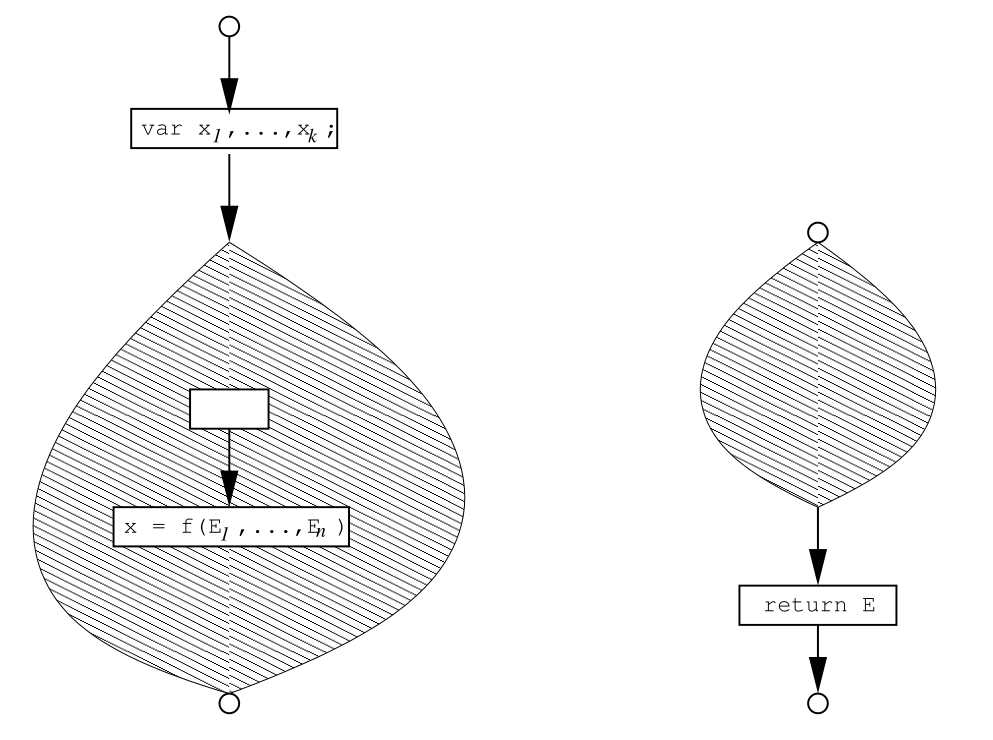
\includegraphics[width=0.6\textwidth]{figures/interprocedural_cfgs}
  \caption{Two CFGs, one for the calling function and one for the called function}
  \label{interprocedural_cfgs}
\end{figure}


\paragraph{Shadow variables}
In order to maintain the correct values for all variables across scopes we introduce \emph{shadow variables}.
Because parameters of functions have no relation to the scope of other functions, parameters can be the same for many different function scopes.
Shadow variables ensure that the meaning of the different scopes are kept when gluing the function CFG into the main CFG.
The process of gluing a function into the calling function can be split up into four steps:
\begin{itemize}
\item When calling a function we need to save the variables of the current scope, ensuring no clashes with the variabels of the function body.
\item Then we need to save all the formal parameters of the function definition and insert the actual parameters into the appropriate variables in order to create the function local scope.
\item The body of the function can now be inserted as it was originally defined, with the exception that all returns need to be assigned to a unique variable.
\item After the function body all the saved variables need to be restored.
\end{itemize}

The final result is a single CFG for the caller with the callee interwoven in.
The result is depicted on \cref{interprocedural_glue}.
Here all the saved variables are characterized with a prefix and a number \emph{i}, which is a unique index for the called function.


\begin{figure}[H]
  \center
  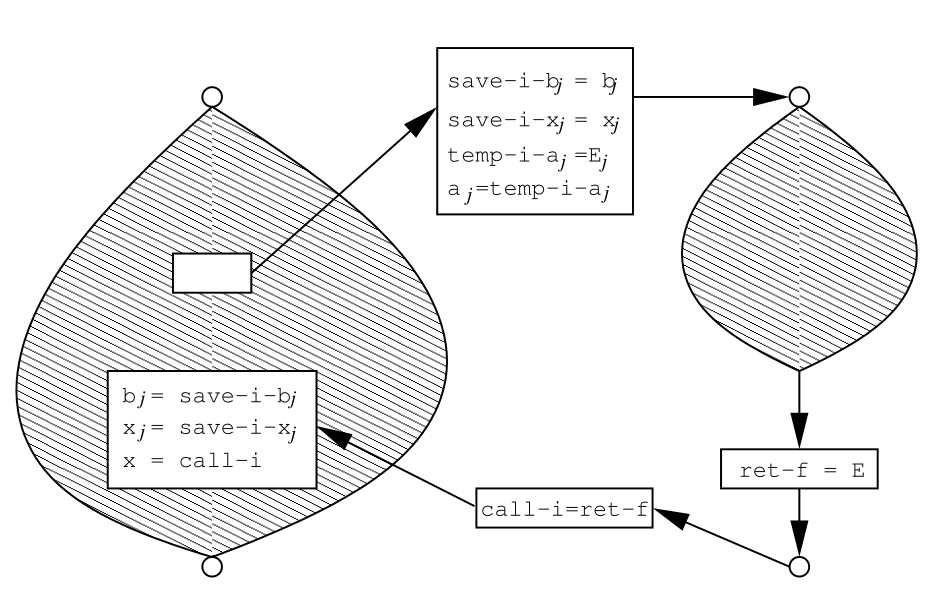
\includegraphics[width=0.6\textwidth]{figures/interprocedural_glue}
  \caption{The two CFGs glued together with shadow variables}
  \label{interprocedural_glue}
\end{figure}

\paragraph{Polyvariance}
If we ``glue in'' the function bodies of called function by referencing the respective CFG, we get a \emph{monovariant} analysis.
An example of monovariant analysis can be seen on \cref{monovariant}
This method has puts some limitiations on the analyses that are performed on the CFG.
For example constant propagation analysis will be inaccurate because more than one call will be represented in the callee CFG.
For our purposes we need propagation of assignments to be accurate for an arbitrary number of calls to a function.

The solution is to make the analysis \emph{polyvariant}.
This is done by make multiple copies of the function body for each call site.
This solves the problem about propagation because every call site has a separate copy of the function where the analysis can perform unique calculations.

\begin{figure}[H]

  \begin{subfigure}[b]{0.49\textwidth}
    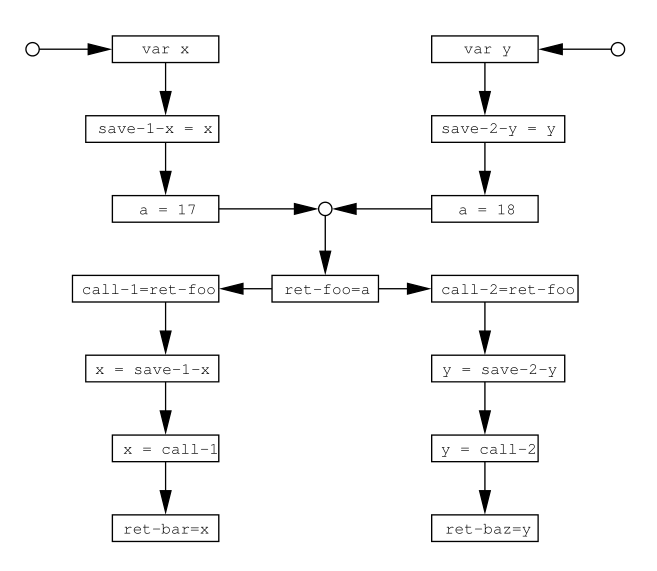
\includegraphics[width=\textwidth]{figures/monovariant}
    \caption{Example CFG of monovariant analysis}
    \label{monovariant}
  \end{subfigure}
 ~ 
  \begin{subfigure}[b]{0.49\textwidth}
    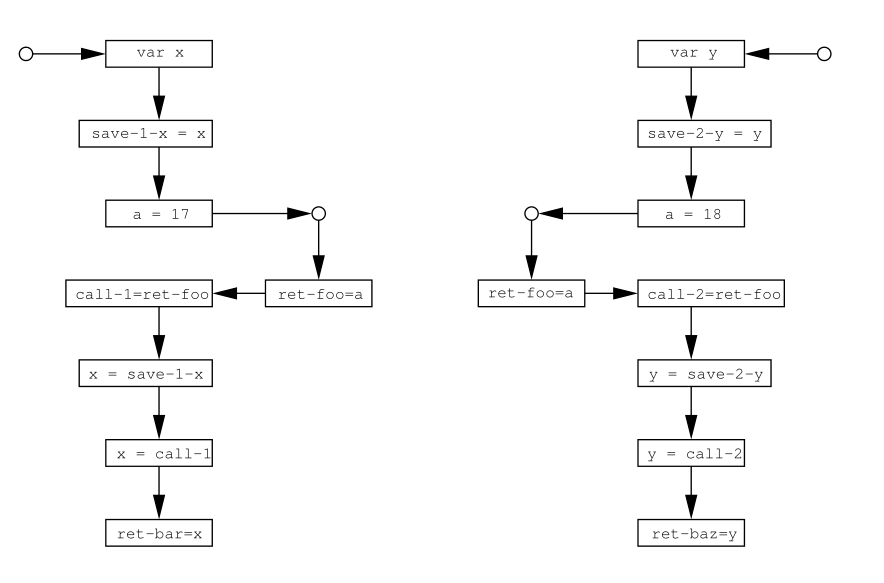
\includegraphics[width=\textwidth]{figures/polyvariant}
    \caption{Example CFG of polyvariant analysis}
    \label{polyvariant}
  \end{subfigure}
  
  \caption{The difference betweem monovariant and polyvariant interprocedural analysis}
  \label{monopoly}
\end{figure}
\todo{the figures use var, do we edit them, footnote or something else?}

\todo{python call by assignment?}
